\documentclass{beamer}
\usepackage[latin1]{inputenc}
%\usetheme{Montpellier}
\usetheme{Boadilla}
%\usecolortheme[RGB={204,51,255}]{structure}
%\usecolortheme[named=purple]{structure}
\usecolortheme[RGB={200,100,50}]{structure}
%\definecolor{dark}{rgb}{0.3,0.15,0.3}
%\definecolor{light}{rgb}{0.8,0.6,0.8}
\definecolor{reddish}{rgb}{.5,0.15,0.15}
\definecolor{dark}{rgb}{0.4,0.2,0.4}
\definecolor{darkgreen}{rgb}{0.25,0.5,0.25}
\definecolor{darkred}{rgb}{0.75,0.25,0.25}
\definecolor{darkblue}{rgb}{0.25,0.25,0.75}
\definecolor{light}{rgb}{0.8,0.6,0.8}
\definecolor{reddish}{rgb}{.7,0.25,0.25}
\usepackage{graphicx}
%\usepackage{pstricks}
\usepackage[normalem]{ulem}

\beamertemplatenavigationsymbolsempty

\usepackage{tikz}
\usetikzlibrary{arrows,decorations.markings,positioning}
\usepackage{epstopdf}

\newcommand*\eiadfamily{\fontencoding{OT1}\fontfamily{eiad}\selectfont}
\usepackage[OT1]{fontenc}

\title[An Ising-like model for language evolution]{An Ising-like model for language evolution}
\author{Conor Houghton}
\date{Labmeeting, May 2022}

\begin{document}

\maketitle




\begin{frame}{Language evolution}
    \begin{minipage}[t][.7\textheight]{\textwidth}
    \vskip 1cm
Does some aspect of the evolution of language lead to the properties of language
\end{minipage}
\end{frame}



\begin{frame}{The iterated language model}
    \begin{minipage}[t][.7\textheight]{\textwidth}
    \vskip 1cm
    \begin{center}
      \includegraphics[width=0.85\textwidth]{ilm.png}
    \end{center}
\end{minipage}
\end{frame}



\begin{frame}{Compositionality}
  \begin{minipage}[t][.7\textheight]{\textwidth}
    \vskip 1cm
    \begin{center}
      \includegraphics[width=0.4\textwidth]{compositional.png}
    \end{center}
\end{minipage}
\vfill
\color{gray}
\flushleft{\small{picture generated by DALL-E}
}
\color{black}
\end{frame}

\begin{frame}{Language change}
  \begin{minipage}[t][.7\textheight]{\textwidth}
    \vskip 1cm
    \begin{center}
      \includegraphics[width=0.3\textwidth]{signs.jpeg}
    \end{center}
\end{minipage}
\vfill
\color{gray}
\flushleft{\small{sign in English, French, G\`{a}idhlig and Mi'kmaw, picture taken from \@{}sadie\_d\_ryan on Twitter}
}
\color{black}
\end{frame}


\begin{frame}{Language change}
  \begin{minipage}[t][.7\textheight]{\textwidth}
    \vskip 1cm
How languages changes, not the evolution of language! A different problem, but maybe one with the same solution; thinking about how languages change now might help us understand the origin of language.
\end{minipage}
\end{frame}


\begin{frame}{Language change - the ILM}
  \begin{minipage}[t][.7\textheight]{\textwidth}
    \vskip 1cm
\textsl{Spatial community structure impedes language amalgamation in a population-based iterated learning model} by George Sains, Conor Houghton and Seth Bullock, accepted for ALIFE 2023.
\end{minipage}
\end{frame}


\begin{frame}{Simplest possible model?}
  \begin{minipage}[t][.7\textheight]{\textwidth}
    \vskip 1cm
    \begin{center}
      \includegraphics[width=0.3\textwidth]{physicists.png}
    \end{center}
\end{minipage}
\vfill
\color{gray}
\flushleft{\small{xkcd.com/793/}
}
\color{black}
\end{frame}

\begin{frame}{Properties of language change?}
  \begin{minipage}[t][.7\textheight]{\textwidth}
    \vskip 1cm
    \begin{itemize}
    \item Agreement supports communication!
    \item Spontaneous change and invention!
    \item An inclination towards consistiency!
      \end{itemize}
  \end{minipage}
\end{frame}


\begin{frame}{Properties of language change?}
  \begin{minipage}[t][.7\textheight]{\textwidth}
    \vskip 1cm
    \begin{itemize}
    \item Agreement supports communication!
    \item Spontaneous change and invention!
    \item \sout{An inclination towards consistiency!}
      \end{itemize}
  \end{minipage}
\end{frame}

\begin{frame}{Idea 1: an Ising model}
  \begin{minipage}[t][.7\textheight]{\textwidth}
    \vskip 1cm
    \begin{center}
      \includegraphics[width=0.4\textwidth]{ising.jpg}
    \end{center}
\end{minipage}
\vfill
\color{gray}
\flushleft{\small{figure from Thermalisation and Relaxation of Quantum Systems, Sascha Wald, 10.13140/RG.2.2.25169.63842}
}
\color{black}
\end{frame}


\begin{frame}{Idea 1: an Ising model}
  \begin{minipage}[t][.7\textheight]{\textwidth}
    \vskip 1cm
\begin{align}
dE&=\frac{2}{n}s_x\sum_y s_y\\
p&=\exp{(-dE/T)}
\end{align}
\end{minipage}
\end{frame}


\begin{frame}{Idea 1: an Ising model}
  \begin{minipage}[t][.7\textheight]{\textwidth}
    \vskip 1cm
    \begin{center}
      \includegraphics[width=0.4\textwidth]{phases.png}
    \end{center}
\end{minipage}
\vfill
\color{gray}
\flushleft{\small{figure from rf.mokslasplius.lt/ising-model/}
}
\color{black}
\end{frame}

\begin{frame}{Language continuum}
  \begin{minipage}[t][.7\textheight]{\textwidth}
    \vskip 1cm
    \begin{center}
      \includegraphics[width=0.6\textwidth]{romance.png}
    \end{center}
\end{minipage}
\vfill
\color{gray}
\flushleft{\small{figure adapted from wikipedia article on dialect continuum}
}
\color{black}
\end{frame}
  

\begin{frame}{Language continuum}
  \begin{minipage}[t][.7\textheight]{\textwidth}
    \vskip 1cm
    \begin{center}
      \includegraphics[width=0.6\textwidth]{romance_basque.png}
    \end{center}
\end{minipage}
\vfill
\color{gray}
\flushleft{\small{figure adapted from wikipedia article on dialect continuum}
}
\color{black}
\end{frame}

\begin{frame}{It's not all continuums}
  \begin{minipage}[t][.7\textheight]{\textwidth}
    \vskip 1cm
    \begin{center}
      \includegraphics[width=0.6\textwidth]{basque_sign.jpeg}
    \end{center}
\end{minipage}
\vfill
\color{gray}
\flushleft{\small{figure from wikipedia article on Gascon}
}
\color{black}
\end{frame}


\begin{frame}{Folks aren't monolingual}
  \begin{minipage}[t][.7\textheight]{\textwidth}
    \vskip 1cm
    \begin{center}
      \includegraphics[width=0.6\textwidth]{kiswahili.png}
    \end{center}
\end{minipage}
\vfill
\color{gray}
\flushleft{\small{figure from wikipedia article on kiSwahili}
}
\color{black}
\end{frame}


\begin{frame}{Idea 2: the Preference Ising model}
  \begin{minipage}[t][.7\textheight]{\textwidth}
    \vskip 1cm
Like the Ising model but only for the neighbour most like you!
\end{minipage}
\end{frame}


\begin{frame}{Idea 2: the Preference Ising model}
  \begin{minipage}[t][.7\textheight]{\textwidth}
    \vskip 1cm
\textsl{An Ising-like model for language evolution} by Conor Houghton accepted for ALIFE 2023
\end{minipage}
\end{frame}

\begin{frame}{The results figure}
  \begin{minipage}[t][.7\textheight]{\textwidth}
    \vskip 1cm
\begin{center}
\includegraphics[height=1.5in]{energy.png}
\end{center}
  \end{minipage}
  \end{frame}


\begin{frame}{The results figure}
  \begin{minipage}[t][.7\textheight]{\textwidth}
    \vskip 1cm
\begin{center}
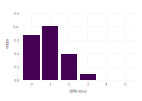
\includegraphics[height=1.5in]{ord_hist.png}
\end{center}
  \end{minipage}
  \end{frame}


\begin{frame}{The results figure}
  \begin{minipage}[t][.7\textheight]{\textwidth}
    \vskip 1cm
\begin{center}
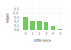
\includegraphics[height=1.5in]{evo_hist.png}
\end{center}
  \end{minipage}
  \end{frame}

\end{document}

